\documentclass[10pt]{beamer}


\usepackage[utf8]{inputenc}
\usetheme{metropolis}
\usepackage{appendixnumberbeamer}
\usepackage[defaultsans]{droidsans}


\usepackage{booktabs}
\usepackage[scale=2]{ccicons}

\usepackage{xspace}
\newcommand{\themename}{\textbf{\textsc{metropolis}}\xspace}

\usepackage{array}


\title{High Level Assembler Plugin}
%\subtitle{Software project}
\date{Supervisor: Miroslav Kratochvíl}
\author{Michal Bali, Marcel Hruška, Peter Polák, Adam Šmelko, Lucia Tódová}
% \institute{Center for modern beamer themes}
% \titlegraphic{\hfill\includegraphics[height=1.5cm]{logo.pdf}}

\begin{document}

\maketitle


\begin{frame}[standout]{Motivation}
\centering
\hspace*{-1cm}
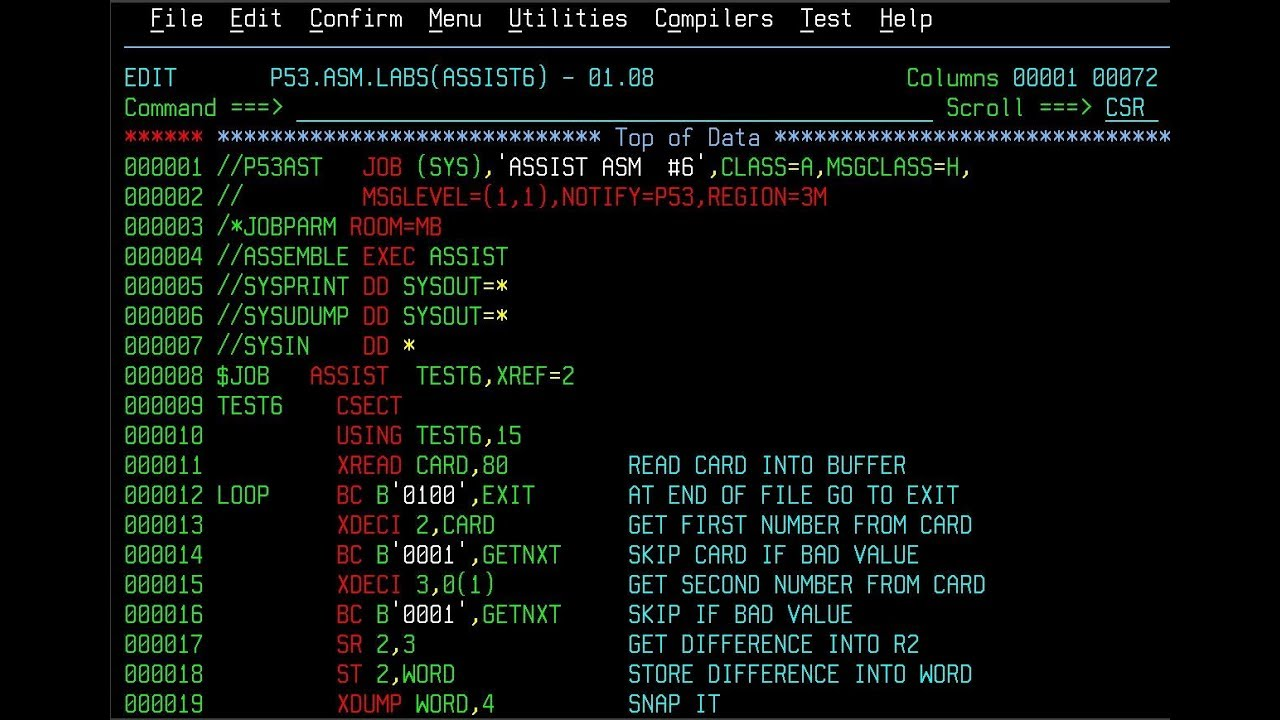
\includegraphics[width=12.6cm]{img/maxresdefault}
\pause
\footnotesize Your Account Balance May Still Rely On Such Code!

\end{frame}

\begin{frame}{Project goals}
    \begin{itemize}
    	\item HLASM support for contemporary source code editors using the Language Server Protocol
    	\item Code validation
    	\item Code navigation (Go to definition, Find all references, \dots)
    	\item Tooltips, autocompletion, \dots
    \end{itemize}

    In the long term:
    \begin{itemize}
        \item Simplify orientation in legacy code
        \item Allow transitioning to some modern language % COBOL
    \end{itemize}
\end{frame}


\begin{frame}{The HLASM language}

There are 3 types of instructions:
\begin{enumerate}
	\item Machine instructions
	\item Assembler instructions \\\quad{\small (`compile'-time variables, modifications of assembler program state)}
	\item Conditional Assembly instructions \\\quad{\small (basically a Turing-complete macro system)}
\end{enumerate}

\textbf{Main problem:} Code interpretation heavily depends on 2.~and 3.

\end{frame}


\begin{frame}[fragile]{Example --- assembler instructions}
  
	\begin{verbatim}
	[00]              LR    1,2
	[01]              DS    CL(LEN)
	[02]   ADDR       DS    CL(SIZE)
	[03]   HERE       DS    CL5
	[04]
	[05]   LEN        EQU   HERE-ADDR
	[06]   SIZE       EQU   1
	\end{verbatim}
	
	Resulting memory layout:
	
	\begin{table}[]
		\begin{tabular}{clll}
			
			\multicolumn{1}{|p{0.5cm}|}{\centering\texttt{2}} & \multicolumn{1}{p{2cm}|}{\centering\texttt{LEN}} & \multicolumn{1}{p{3cm}|}{\centering\texttt{SIZE}} & \multicolumn{1}{p{1.5cm}|}{\centering\texttt{5}}  \\ \hline
			 &   & \multicolumn{1}{l}{\hspace{-10pt}\rotatebox{90}{\texttt{ADDR->} }}  & \multicolumn{1}{l}{\hspace{-10pt}\rotatebox{90}{\texttt{HERE->}}}                       
		\end{tabular}
	\end{table}
	
\end{frame}

\begin{frame}[fragile]{Example --- Conditional Assembly}


\begin{verbatim}
	[00]   &VAR       SETA    1
	[01]   .LOOP      ANOP         
	[02]   SYM        DC      &VAR.C'A'
	[03]              AIF     (L'SYM GE 10).END
	[04]              MAC     &VAR
	[06]   &VAR       SETA    &VAR+1
	[07]              AIF     (&VAR LE 5).LOOP
	[08]   .END       END     
\end{verbatim}

\end{frame}

\begin{frame}{Architecture}
\centering
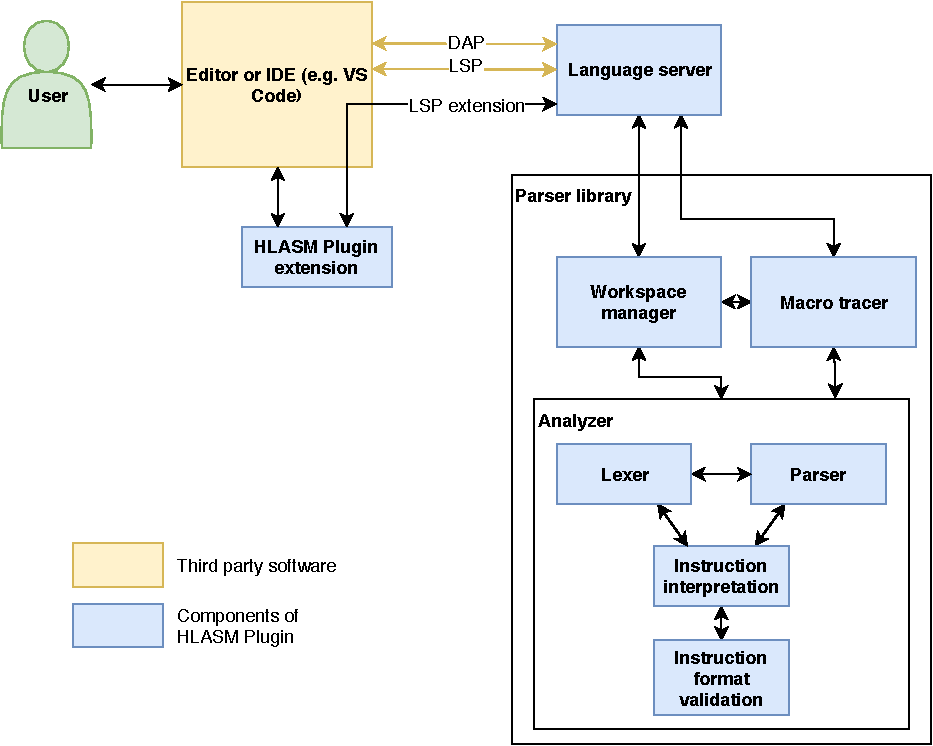
\includegraphics[width=10.5cm]{img/hlasm_architecture}
\end{frame}


\begin{frame}{Already done: Preview version}
\centering
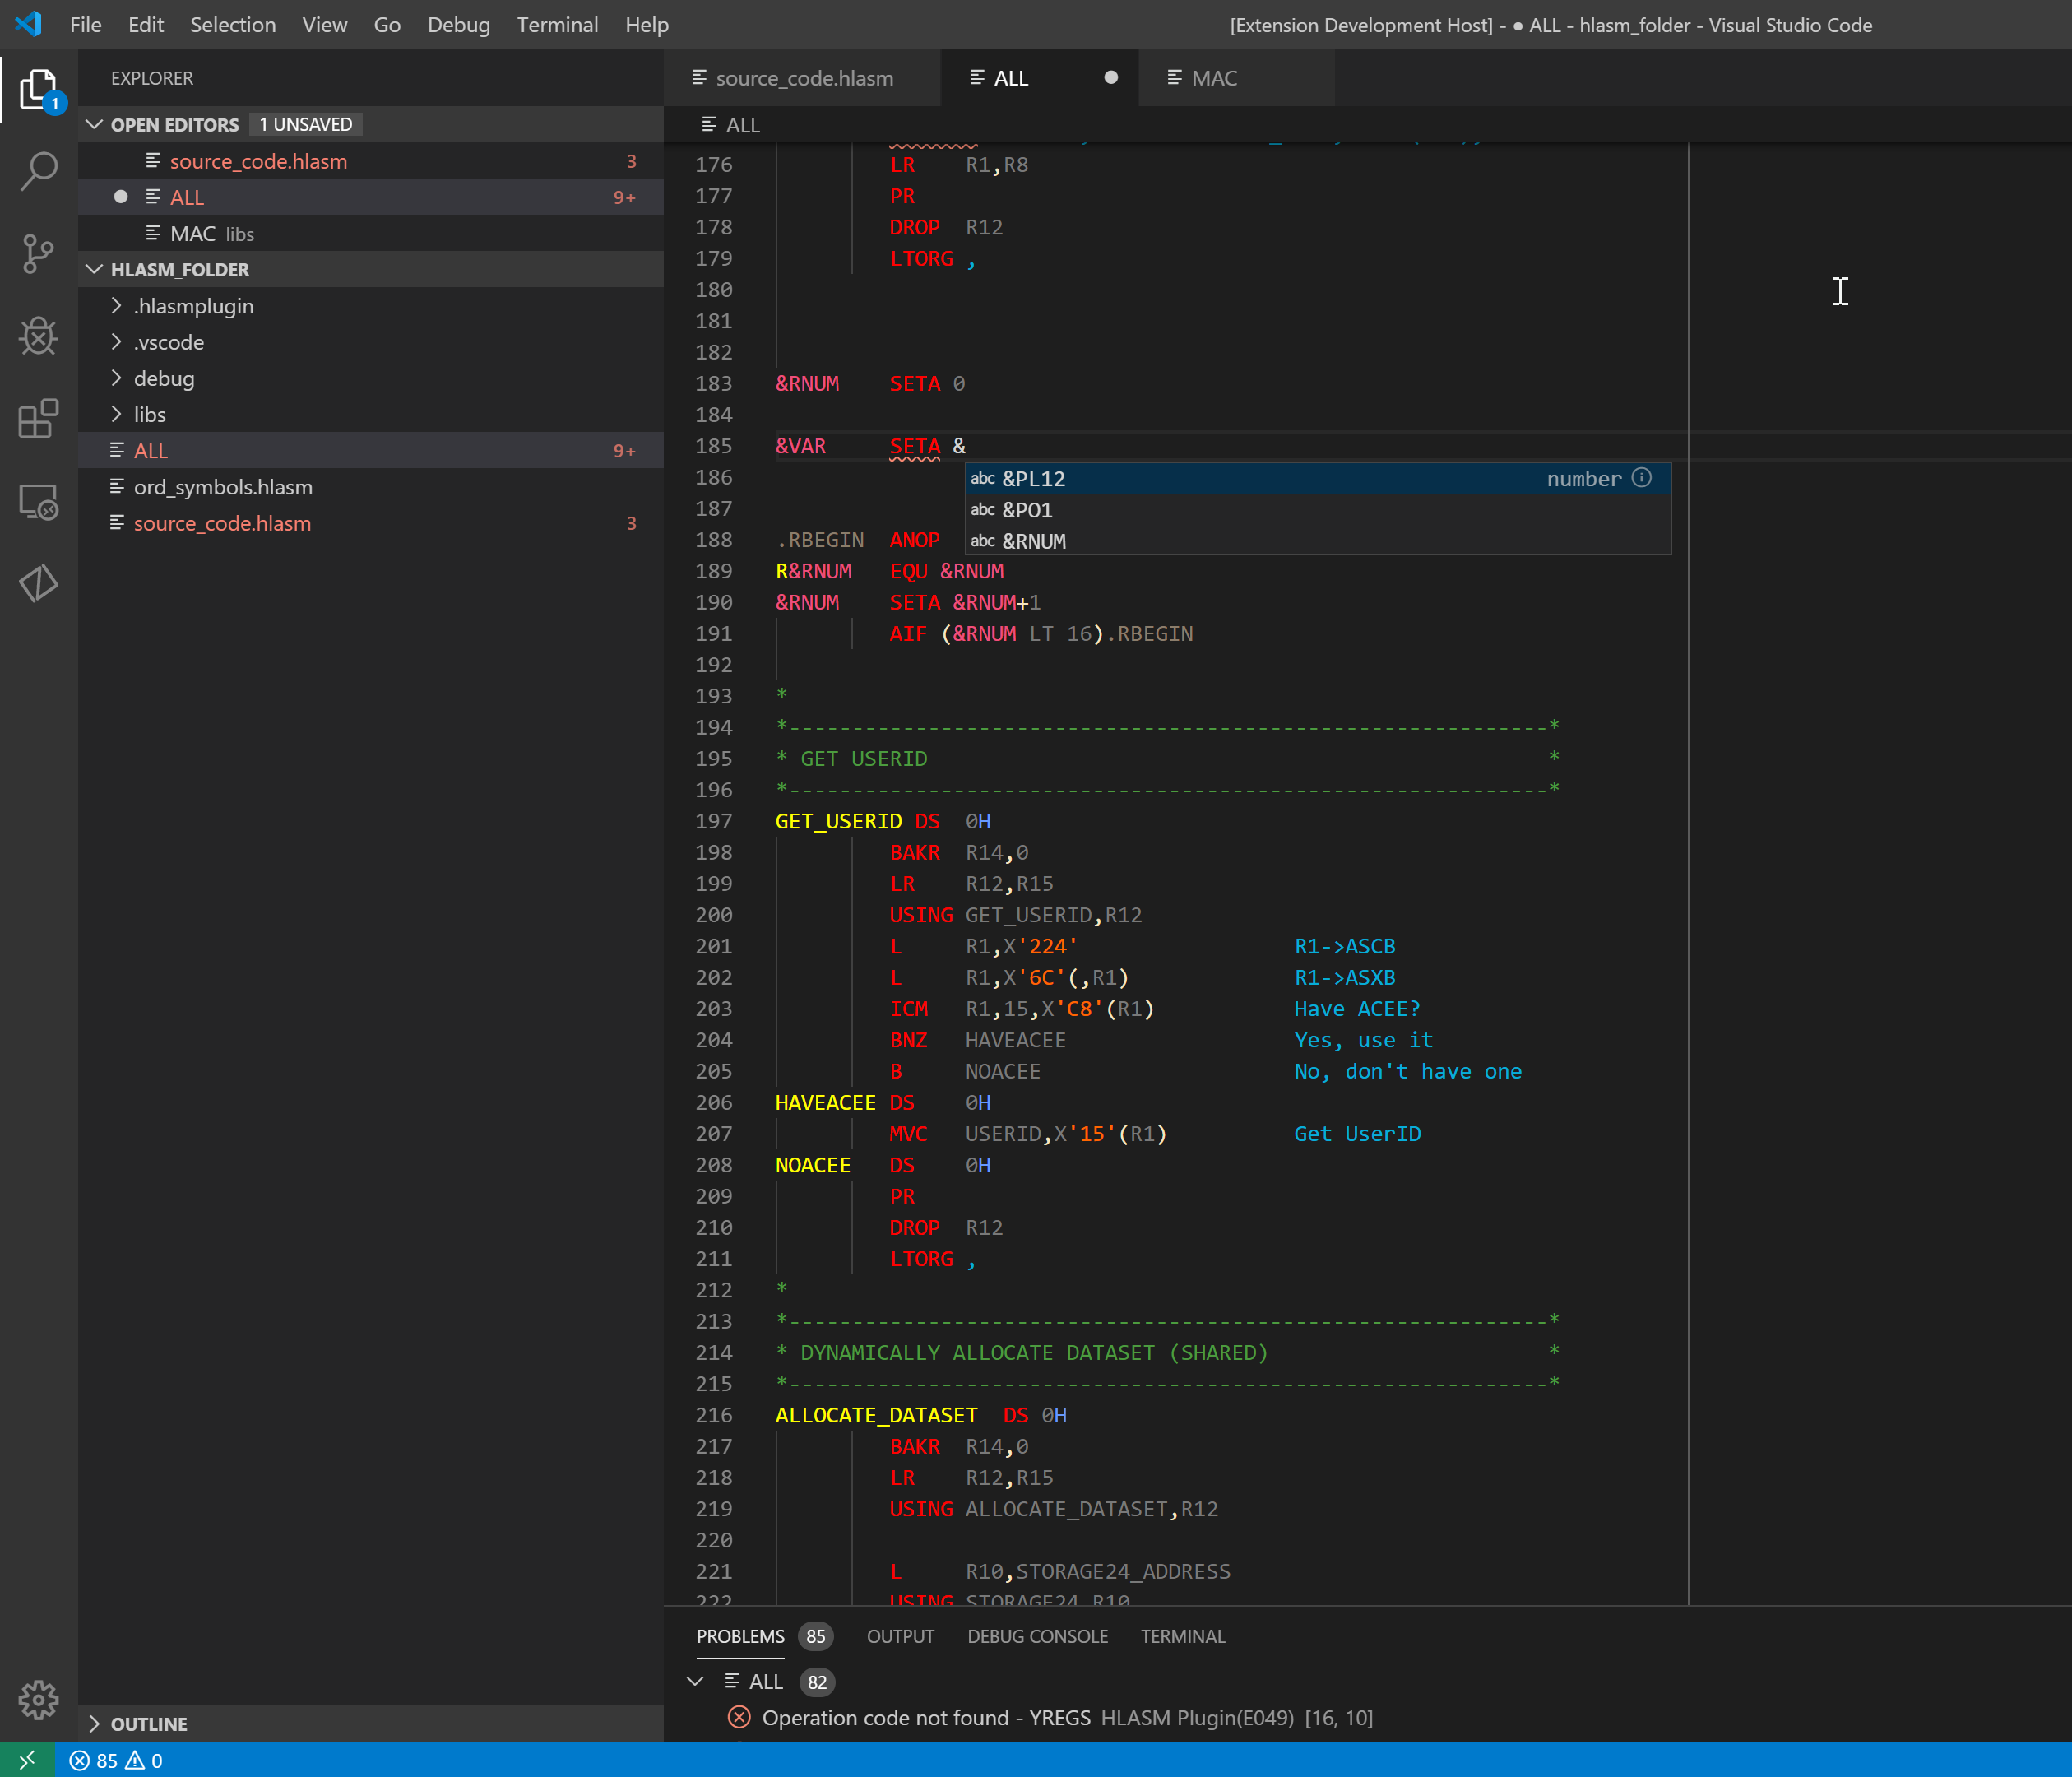
\includegraphics[width=9cm]{img/screenshot}

\footnotesize
Source code taken from \url{https://github.com/zhaimlill/EnhanceStartOnZ}
\end{frame}


\begin{frame}{Current timeline}

\centering
\hspace*{-0.95cm}
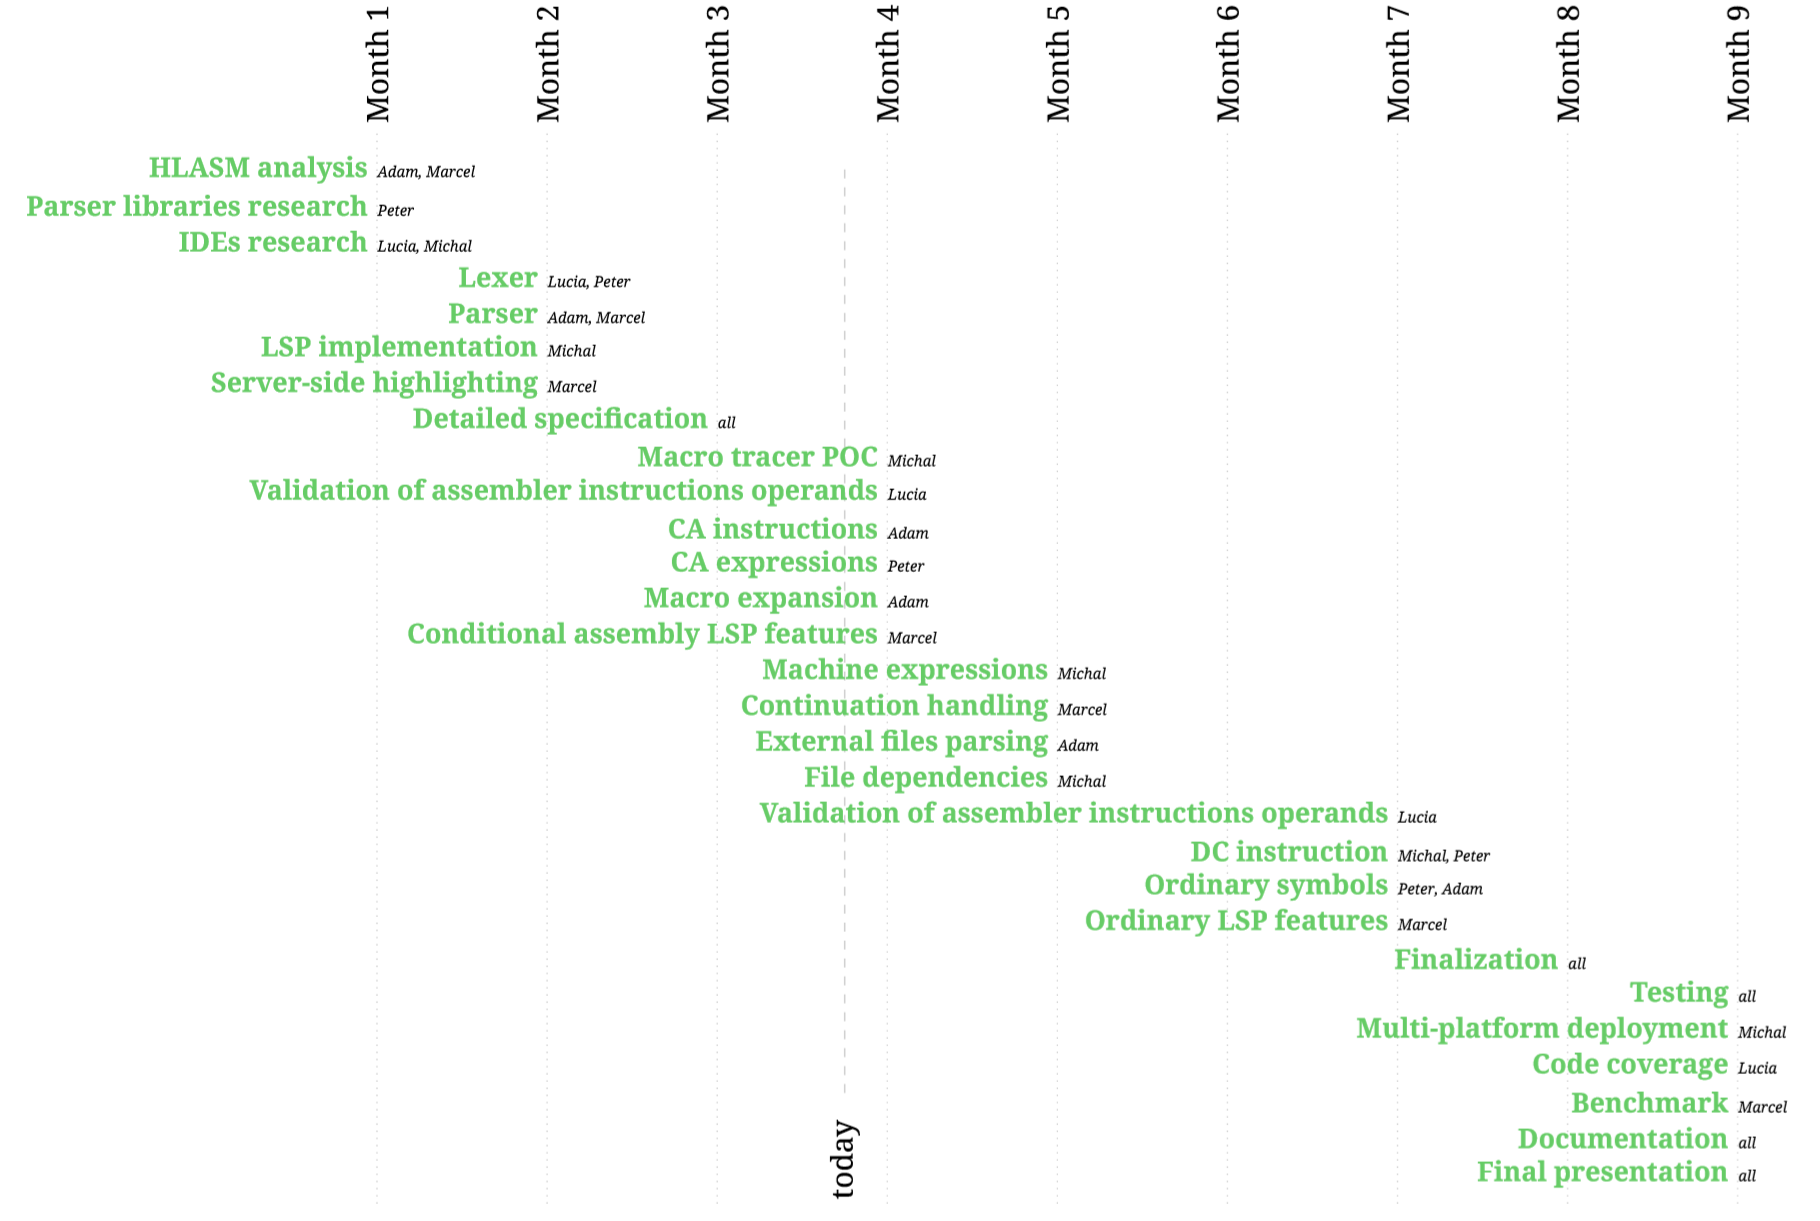
\includegraphics[width=12.5cm]{img/timeline}

\end{frame}


\begin{frame}[standout]

  Thank you for attention.

  \small Questions?
\end{frame}


\end{document}
